割点

> 对于一个无向图,如果把一个点删除后这个图的极大连通分量数增加了,那么这个点就是这个图的割点(又称割顶)。

如何实现?

如果我们尝试删除每个点,并且判断这个图的连通性,那么复杂度会特别的高。所以要介绍一个常用的算法:Tarjan。

首先,我们上一个图:

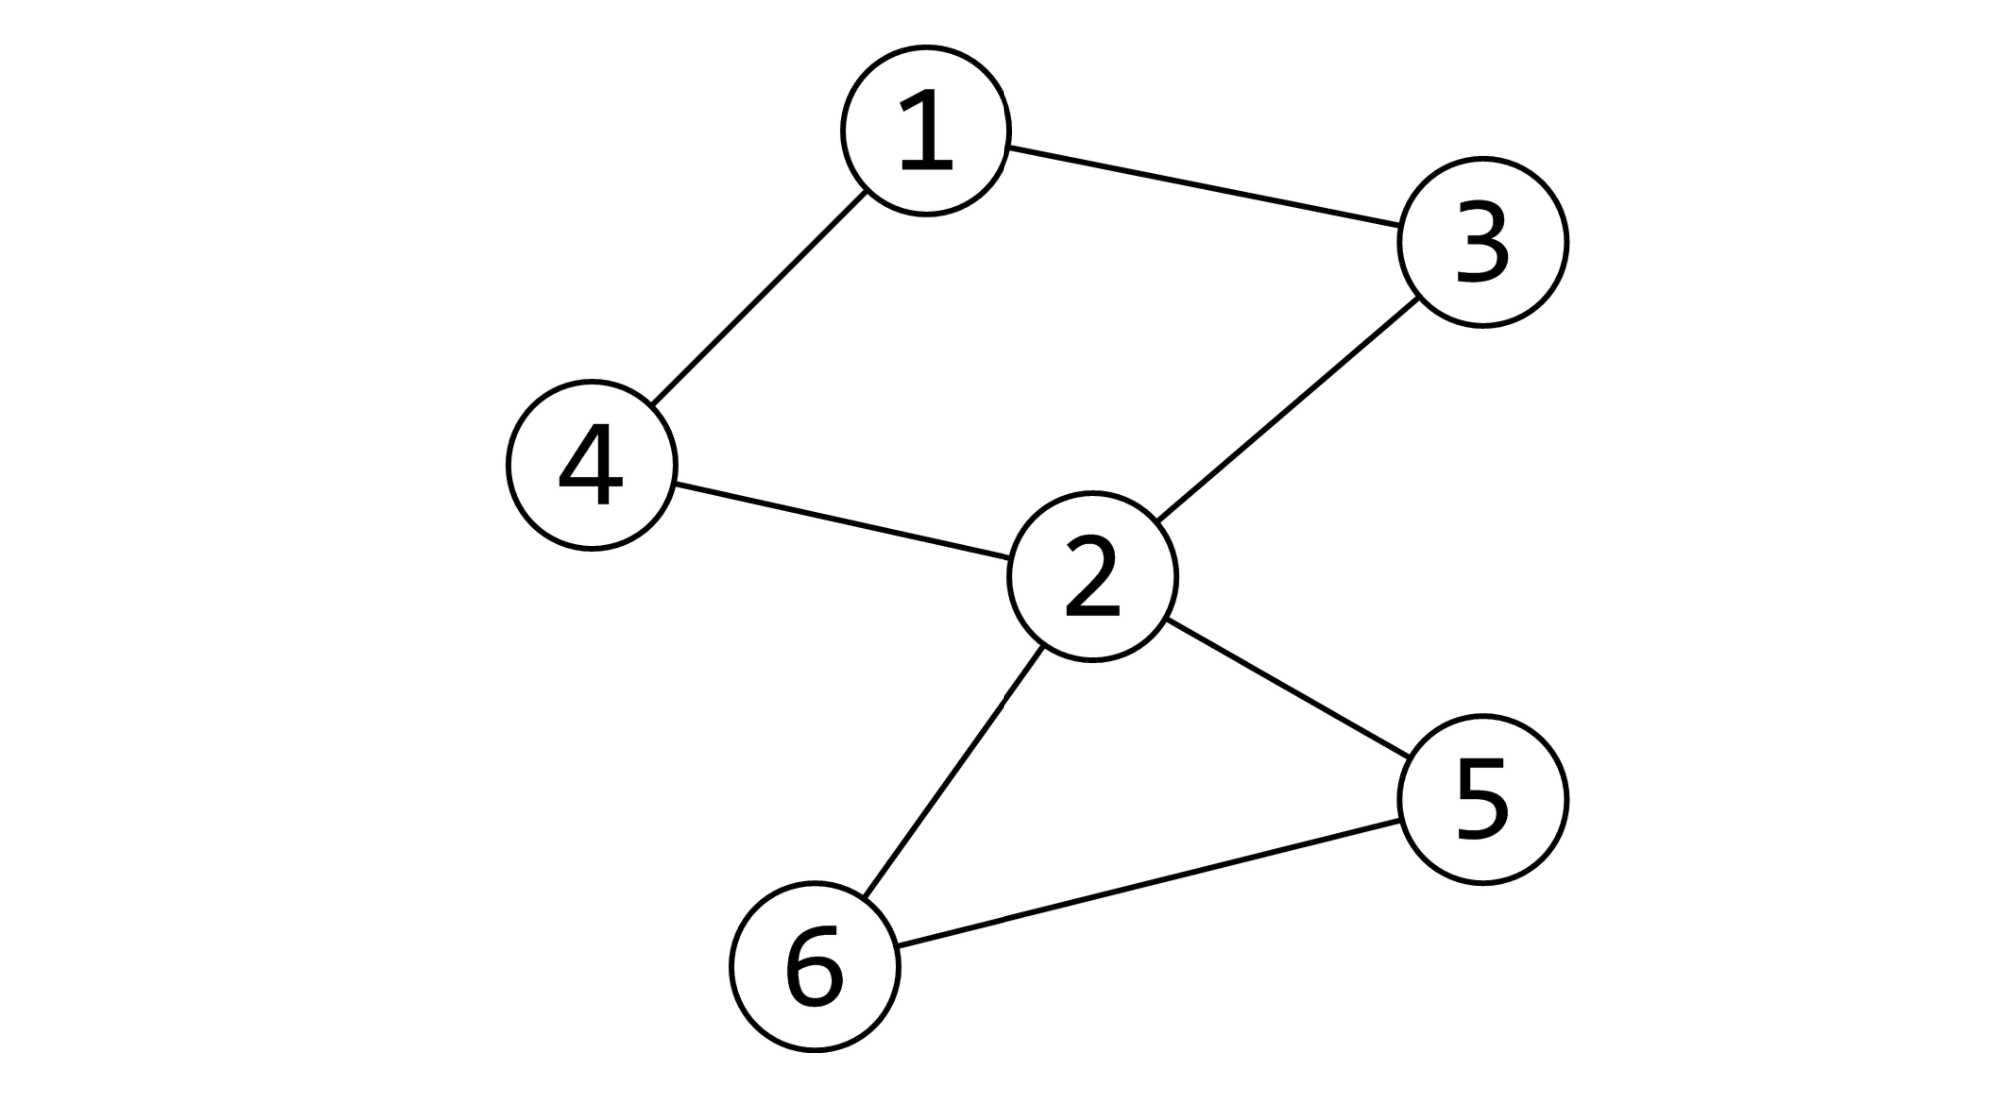
\includegraphics[width=0.95\textwidth]{D:/ACM/代码模板/ver6.0/ICPC-Code-Template-in-Latex/图论/tarjan/bridge1.png}

很容易的看出割点是 2,而且这个图仅有这一个割点。

首先,我们按照 DFS 序给他打上时间戳(访问的顺序)。

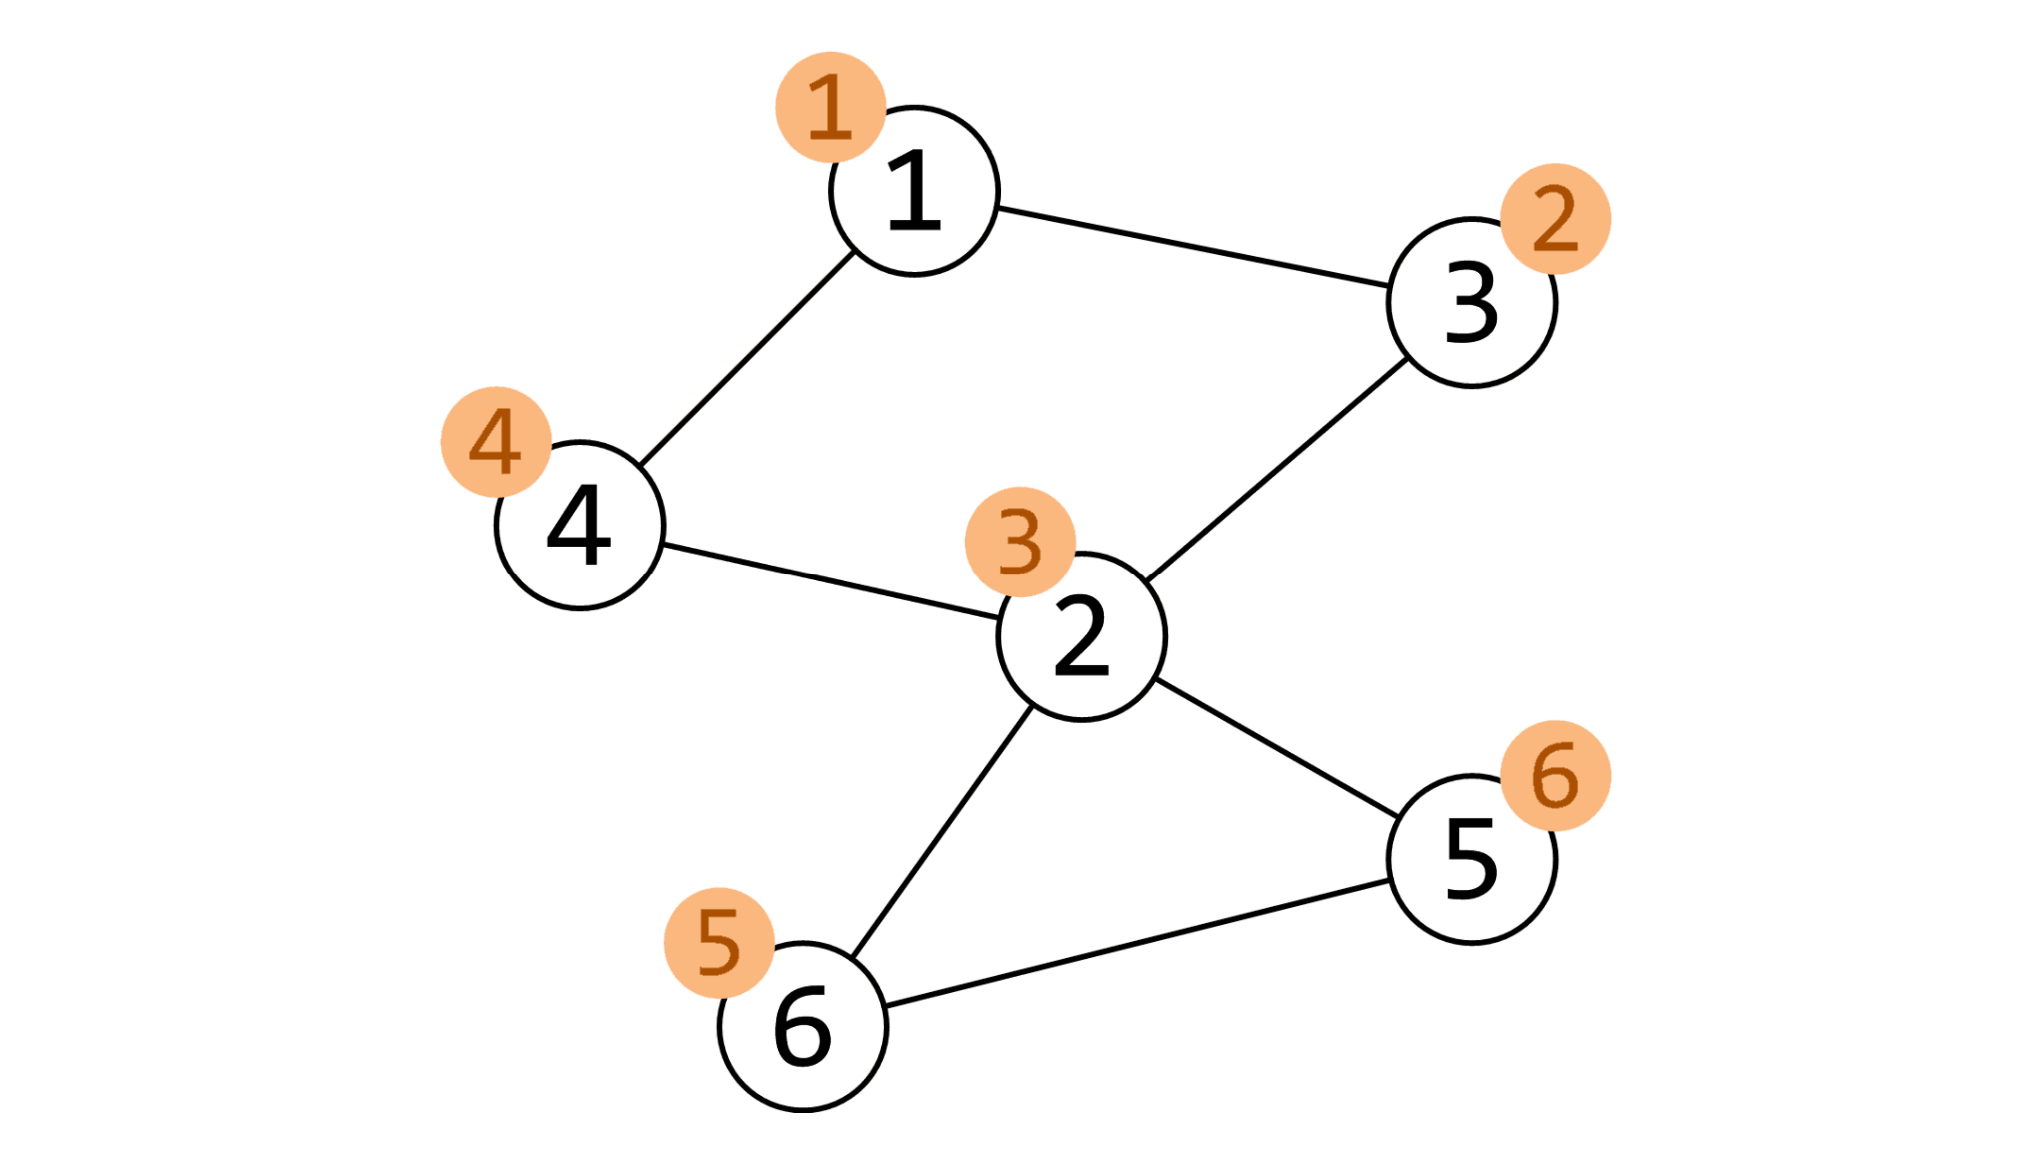
\includegraphics[width=0.95\textwidth]{D:/ACM/代码模板/ver6.0/ICPC-Code-Template-in-Latex/图论/tarjan/bridge2.png}

这些信息被我们保存在一个叫做 `num` 的数组中。

还需要另外一个数组 low ,用它来存储不经过其父亲能到达的最小的时间戳。

例如low[2] 的话是 1, low[5] 和 low[6] 是 3。

然后我们开始 DFS,我们判断某个点是否是割点的根据是:对于某个顶点 $u$ ,如果存在至少一个顶点 $v$ ( $u$ 的儿子),使得 $low_v \geq num_u$ ,即不能回到祖先,那么 $u$ 点为割点。

另外,如果搜到了自己(在环中),如果他有两个及以上的儿子,那么他一定是割点了,如果只有一个儿子,那么把它删掉,不会有任何的影响。比如下面这个图,此处形成了一个环,从树上来讲它有 2 个儿子:

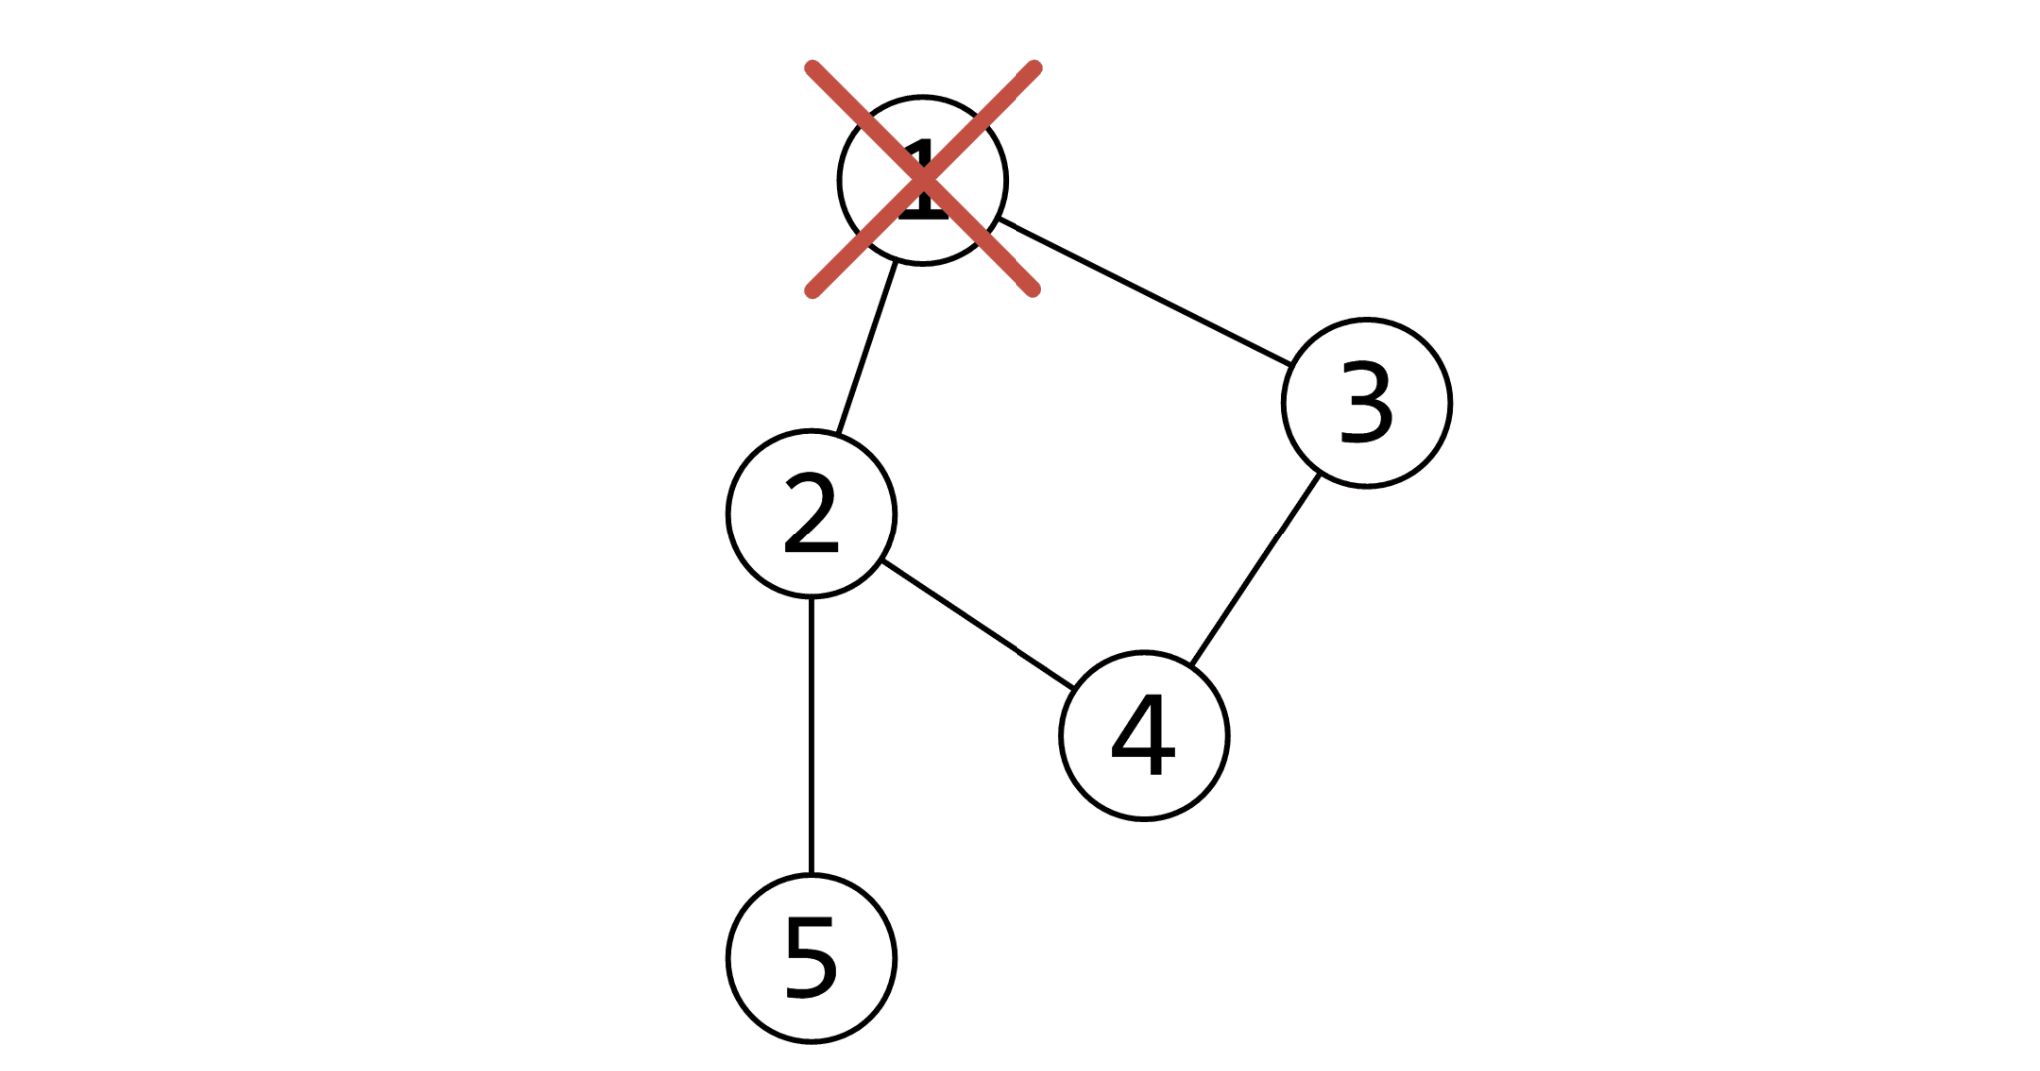
\includegraphics[width=0.95\textwidth]{D:/ACM/代码模板/ver6.0/ICPC-Code-Template-in-Latex/图论/tarjan/bridge3.png}

我们在访问 1 的儿子时候,假设先 DFS 到了 2,然后标记用过,然后递归往下,来到了 4,4 又来到了 3,当递归回溯的时候,会发现 3 已经被访问过了,所以不是割点。

更新low的伪代码如下:

\begin{lstlisting}
如果 v 是 u 的儿子 low[u] = min(low[u], low[v]);
否则
low[u] = min(low[u], num[v]);
\end{lstlisting}


例题
洛谷 P3388【模板】割点(割顶)
